\documentclass[11pt,a4paper]{article}
\usepackage[utf8]{inputenc}
\usepackage[T1]{fontenc}
\usepackage{amsfonts}
\usepackage[french]{babel}
\frenchbsetup{StandardLists=true} % à inclure si on utilise \usepackage[francais]{babel}
\usepackage{enumitem}
\usepackage{amssymb}
\usepackage{amsmath}
\usepackage[left=2cm,right=2cm,top=2cm,bottom=2cm]{geometry}
\usepackage{multirow}
\usepackage[dvipsnames]{xcolor}

\usepackage[T1]{fontenc}
\usepackage{fouriernc}
\usepackage{graphicx}

%\usepackage{setspace}
%\singlespacing

\usepackage{pstricks}
\usepackage{xkeyval}
\usepackage{pst-labo}


\usepackage{multicol}
\setlength{\columnsep}{1cm}
\usepackage{caption}
\usepackage{fancyhdr}
\pagestyle{fancy}
\renewcommand\headrulewidth{1pt}
\fancyhead[L]{Lycée Denis Diderot }
\fancyhead[R]{Classe de 1 Bac Pro }
\setcounter{page}{4}\fancyfoot[C]{page \thepage}
\fancyfoot[R]{Année 2024-2025}
\fancyfoot[L]{Alexis RUIZ}
\usepackage{multirow,tabularx,booktabs}
\usepackage[tikz]{bclogo} 
\usepackage{qrcode}

\newcommand{\cadreblanc}[1]{%
\medskip\framebox[\linewidth][c]{%
\rule{0mm}{#1mm}}\par
\medskip}

\usepackage{awesomebox}
\setlength{\aweboxvskip}{0mm}
\usepackage{pifont}
\usepackage{chemmacros}
\chemsetup{modules=all}
\setlength{\columnseprule}{.25mm}


% Couleurs personnalisées
\definecolor{darkblue}{RGB}{0,51,102}
\definecolor{lightblue}{RGB}{173,216,230}
\definecolor{graybox}{RGB}{240,240,240}




\renewcommand{\arraystretch}{1.5}
\newcommand*\acocher{\quitvmode{\fboxsep0pt \fboxrule0.8pt \fbox{\vrule height1.8ex depth.1ex width0pt \vrule height0pt depth0pt width1.9ex }}}

\newcolumntype{C}[1]{>{\centering\arraybackslash }b{#1}}

\newcommand{\code}{\awesomebox[black]{2pt}{

\includegraphics[scale=0.15]{../Chapitre 1 - Energie et puissance électrique/images/frame.png}
}{black}}

\newcommand{\moteur}{\awesomebox[black]{2pt}{

\includegraphics[scale=1]{images/moteur.jpg} 
}{black}}

\newcommand{\defconclusion}{\awesomebox[black]{2pt}{\rotatebox{90}{\Large{\textbf{Conclusion}}}}{black}}

\newcommand{\defbox}{\awesomebox[black]{2pt}{
\includegraphics[scale=0.5]{../Chapitre 1 - Energie et puissance électrique/images/appel exam.png}}{black}}

  \newenvironment{itemize*}%  % listes compactes
    {\begin{itemize}%
      \setlength{\itemsep}{0pt}%
      \setlength{\parskip}{0pt}}%
    {\end{itemize}}

\frenchbsetup{StandardLists=true}

\usepackage{tcolorbox}
\tcbuselibrary{skins,breakable}


\begin{document}


% Configuration des boîtes tcolorbox


\flushleft \textbf{NOM : \hfill Classe : \hspace{3cm} ~~\\[2mm]
Prénom:\\[0,4cm]
}
\hrule\
%\\[0,1cm]

\begin{center}
 \LARGE{TP - Étude de la chute libre d'une balle  }
\end{center}

%\vspace{2 mm}

\normalsize

\hrule\
\\[0,2cm]
   \begin{center}
   \textbf{Le soin et la rédaction interviendront dans la notation.}
   \end{center} 

\noindent%
\begin{minipage}{.35\textwidth}%

    
 \begin{bclogo}[couleur=blue!30 ,  arrondi =0.1 , logo = \bcinfo, epBarre =2]{ Matériel }

\begin{itemize*}
    \item 1 smartphone 
    \item 1 calculatrice


\end{itemize*}
\end{bclogo}

\end{minipage}%
\hfill 
\begin{minipage}{.6\textwidth}%
\begin{center}

    \item Télécharger l'application Fizziq sur votre téléphone. \\

    
 


     \begin{tabular}{cc}
         Android & IOS\\
          \qrcode{https://play.google.com/store/apps/details?id=com.chazot.fizziq&hl=fr} & \qrcode{https://apps.apple.com/fr/app/fizziq/id1516870599}\\
     \end{tabular}





\end{center}
\end{minipage}%

\vfill 


\fcolorbox{black}{blue!30}{\textbf{Protocole}}


Ouvrir l'application Fizziq puis choisir d' importer la vidéo "Chute libre" : \\[2mm]


\noindent%
\begin{minipage}{.2\textwidth}%
\begin{center}
Analyse\\cinématique 
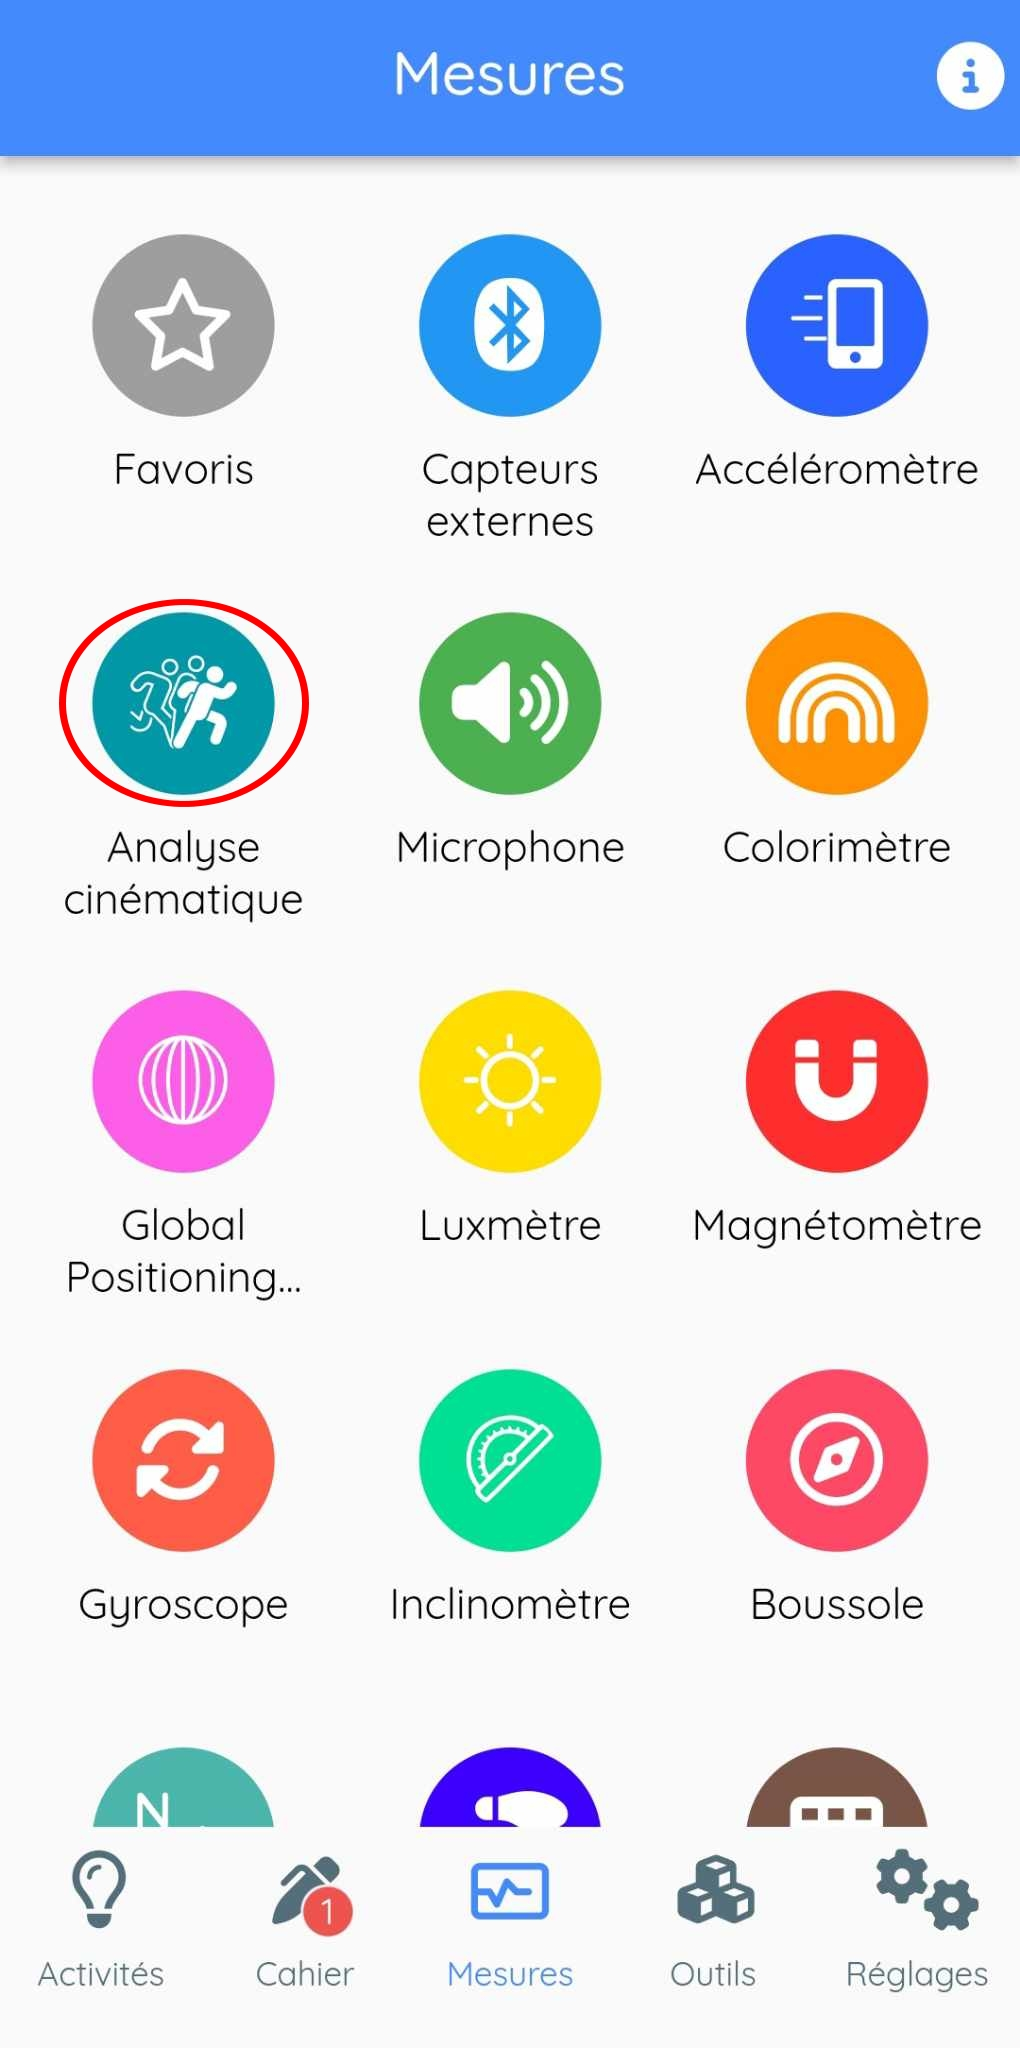
\includegraphics[width=\textwidth]{images/1.jpg}
\end{center}
\end{minipage}%
\hfill
\begin{minipage}{.2\textwidth}%
\begin{center}
Cinématique \\par vidéo 
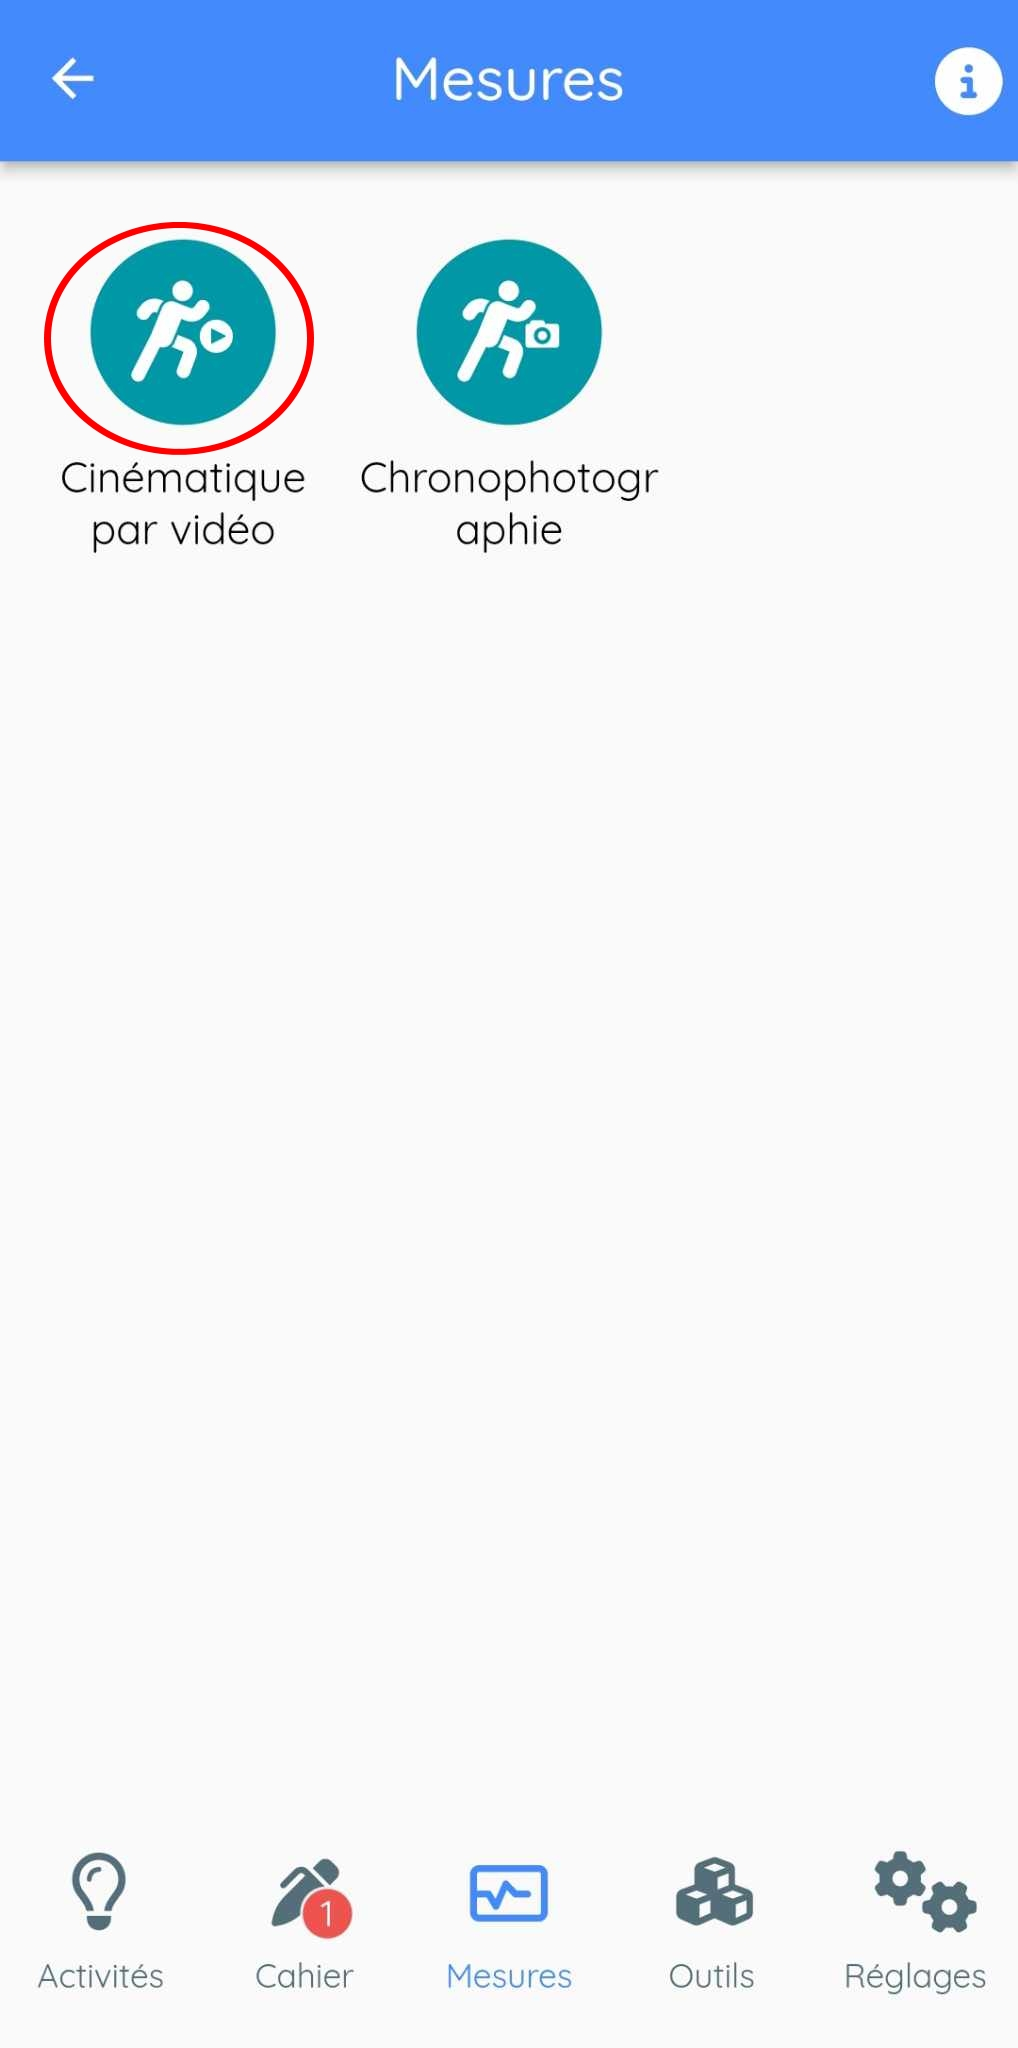
\includegraphics[width=\textwidth]{images/2.jpg}
\end{center}
\end{minipage}%
\hfill
\begin{minipage}{.20\textwidth}%
\begin{center}
Chute libre
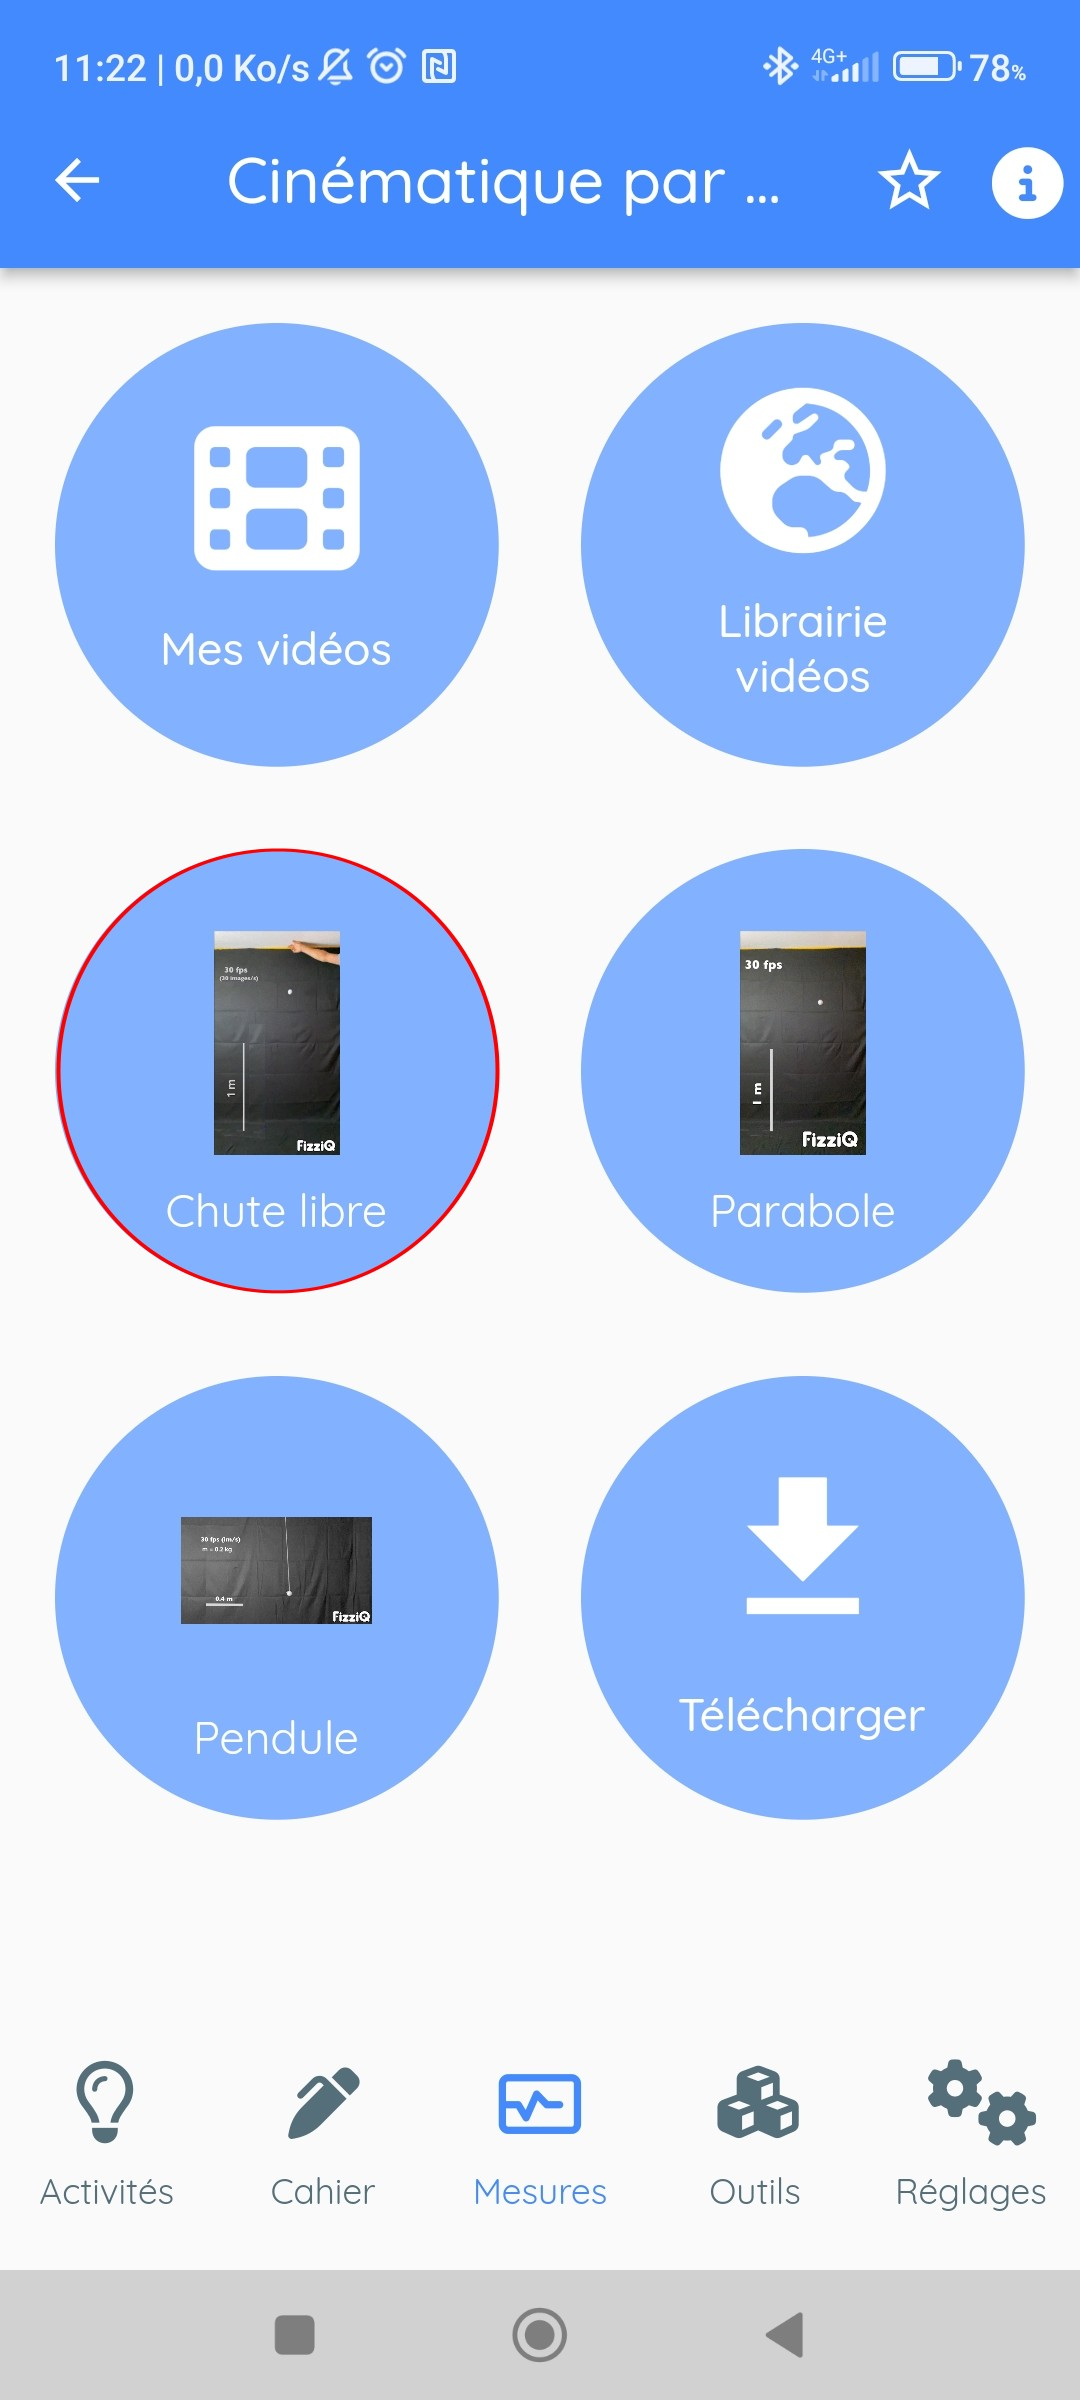
\includegraphics[width=\textwidth]{images/32.jpg}
\end{center}
\end{minipage}%


\vfill  


    \begin{multicols}{2}


\item Réglage de la longueur de la règle : \\[5mm]
\begin{itemize}
    \item Sur la nouvelle fenêtre, positionner l'origine du repère sur le centre de la balle. Régler celle-ci afin qu'elle mesure 1m. Le repère sera orienté dans le sens du mouvement. 
    \item Préciser dans la fenêtre en haut à gauche la longueur de la règle en m ; 1m. 

\end{itemize}



\columnbreak

\item Sélectionner Pointage : 
\begin{itemize}
    \item Laisser l'intervalle de temps $\mathrm{\Delta t ~à~33 ms}$
    \item Positionner la mire au centre de la balle et cliquer. 
    \item La vidéo passe alors à l'image suivante. Recommencer l'opération pour avoir au moins 15 points.  
\end{itemize}

\end{multicols}

\vfill 


\newpage


\fcolorbox{black}{blue!30}{\textbf{Mesures}}\\
\ding{202} Aller dans résultats, cocher T(s), le temps en secondes et y(m), la distance en mètre. \\Compléter le tableau suivant : 

\begin{center}
    
\renewcommand{\arraystretch}{1.8}
    \begin{tabular}{|C{3cm}||C{0.5cm}|C{0.5cm}|C{0.5cm}|C{0.5cm}|C{0.5cm}|C{0.5cm}|C{0.5cm}|C{0.5cm}|C{0.5cm}|C{0.5cm}|C{0.5cm}|C{0.5cm}|C{0.5cm}|C{0.5cm}|C{0.5cm}|}
         \hline
         Point ($i$) & 1 &  2& 3 & 4 & 5 & 6& 7& 8& 9 & 10& 11 & 12 & 13 & 14 & 15\\
         \hline
         $t_i(s)$ &  &  &  &  &  & & & & & & & & & & \\
         \hline
          $y_i(m)$ &  &  &  & & & & & & & & & & & & \\
         \hline
 
    \end{tabular}

    \end{center}


\ding{203} Compléter le graphique en utilisant les valeurs du tableau. 


\begin{center}
    
\begin{tikzpicture}[scale=0.8]
%papier milli
\draw [very thin, orange!20] (0,-3) grid[step=0.1] (16,5);

\draw [very thin, blue!20] (0,-3) grid[step=0.5] (16,5);
\draw [very thin, black!40] (0,-3) grid[step=1] (16,5);
\draw[->,>=stealth] (0,-3) -- (16.3,-3) node[below right] {$t_i(s)$};
%stealth définit un style de flèche, "furtif"
\draw[->,>=stealth] (0,-3) -- (0,5.3)node[below left] {$y_i (m)$};

\draw (0,-2.9) -- (0,-3.1) node [below] {{\scriptsize $t_1$}}; 

\draw (1,-2.9) -- (1,-3.1) node [below] {{\scriptsize $t_2$}}; 

\draw (2,-2.9) -- (2,-3.1) node [below] {{\scriptsize $t_3$}}; 

\draw (0,-3) -- (-0.10,-3) node [left] {{\scriptsize $0$}}; 

\draw (0,-2) -- (-0.10,-2) node [left] {{\scriptsize $0,2$}}; 



\end{tikzpicture}



\begin{minipage}{0.9\textwidth}%

    

 
 \begin{bclogo}[couleur=blue!30 ,  arrondi =0.1 , logo = \bcinfo, epBarre =2]{ Calcul de la vitesse }
\begin{center}
    

 Pour la calculer la vitesse instantanée au point $i$, on calcule la vitesse entre les points $i-1$ et $i+1$. \\[0.3cm]
 

 Ce qui nous donne : $v_i=\dfrac{y_{i+1}-y_{i-1}}{t_{i+1}-t_{i-1}}$   
\hspace{2cm}
 Exemple en $i=2$ , $v_2=\dfrac{y_{3}-y_{1}}{t_{3}-t_{1}}$ \\[0.3cm]

 Remarque : en utilisant cette méthode , on ne peut calculer $v_0$ et $v_{15}$

 \end{center}
\end{bclogo}

\end{minipage}
\end{center}


\ding{203} Compléter le tableau suivant : 
    
\renewcommand{\arraystretch}{1.8}
    \begin{tabular}{|C{3cm}||C{0.5cm}|C{0.5cm}|C{0.5cm}|C{0.5cm}|C{0.5cm}|C{0.5cm}|C{0.5cm}|C{0.5cm}|C{0.5cm}|C{0.5cm}|C{0.5cm}|C{0.5cm}|C{0.5cm}|C{0.5cm}|C{0.5cm}|}
         \hline
         Point ($i$) & 1 &  2& 3 & 4 & 5 & 6& 7& 8& 9 & 10& 11 & 12 & 13 & 14 & 15\\
         \hline
         
         $y_i(m)$ &  &  &  & & & & & & & & & & & & \\
         \hline 
         
          $y_{i+1}-y_{i-1}~~(m)$ &  &  &  & & & & & & & & & & & & \\
           \hline
           $t_i(s)$ &  &  &  &  &  &  & &  &  &  & & & & &  \\
         \hline
         $t_{i+1}-t_{i-1}~~(s)$ &  &  &  &  &  & & & & & & & & & & \\
         \hline
          $v_i(m/s)$ &  &  &  & & & & & & & & & & & & \\
          \hline
         
 
    \end{tabular}

    \vspace{5mm}

    \ding{207} La vitesse : \hspace{5mm} $\square$~augmente \hspace{3cm} $\square$~reste constante\hspace{3cm} $\square$~diminue


\vfill

\newpage


\ding{203} Compléter le graphique en utilisant les valeurs du tableau $(t_i ; v_i)$


\begin{center}
    
\begin{tikzpicture}[scale=1]
%papier milli
\draw [very thin, orange!20] (0,-3) grid[step=0.1] (15,9);

\draw [very thin, blue!20] (0,-3) grid[step=0.5] (15,9);
\draw [very thin, black!40] (0,-3) grid[step=1] (15,9);
\draw[->,>=stealth] (0,-3) -- (15.5,-3) node[below right] {$t_i(s)$};
%stealth définit un style de flèche, "furtif"
\draw[->,>=stealth] (0,-3) -- (0,9.5)node[below left] {$v_i~(m/s)$};

%\draw (0,-2.9) -- (0,-3.1) node [below right] {{\scriptsize $t_1$}}; 

\draw (0,-3) -- (-0.10,-3) node [left] {{\scriptsize $0$}}; 

\draw (0,-2.9) -- (0,-3.1) node [below] {{\scriptsize $t_1$}}; %échelle abscisse 

\draw (1,-2.9) -- (1,-3.1) node [below] {{\scriptsize $t_2$}}; %échelle abscisse 

\draw (0.1,-2) -- (-0.1,-2) node [left] {{\scriptsize 0,5}}; %échelle ordonnée 

\end{tikzpicture}
\end{center}






\fcolorbox{black}{blue!30}{\textbf{Interprétation }} \\[5mm]
\ding{205} Commentez la représentation graphique que vous avez obtenue. \\



\cadreblanc{10}

\vfill 

\ding{206} Que peut-on dire de $v$ par rapport à $t$ ? \\
\vspace{5mm}
\dotfill

\vfill 

\ding{208} \'A l'aide de la calculatrice , déterminer l'équation de la droite (Voir tuto calculatrice à la dernière page) \\
\vspace{5mm}
\dotfill

\vfill 

\ding{209} Comparer la valeur du coefficient directeur la droite de régression à l'accélération de la pesanteur , $g=9,81~m/s^2$ \\ 
\vspace{5mm}
\dotfill




\vfill 

\newpage



\begin{center}
    \begin{tcolorbox}[colback=darkblue!10, colframe=darkblue, width=\textwidth, arc=2mm, boxrule=1pt]
        \begin{center}
            \Large{\textbf{Statistiques à deux variables}} \\[0.2cm]
            \large{Calcul des paramètres statistiques, régression} \\[0.1cm]
            \textbf{TI 82 Stats.fr}
        \end{center}
    \end{tcolorbox}
\end{center}

\vspace{0.2cm}

\begin{tcolorbox}[colback=lightblue!20, colframe=darkblue, title=\textbf{Objectifs}, arc=2mm, boxrule=0.8pt]
    \small
    \textbf{1)} Déterminer les éléments caractéristiques de chaque série. \\[0.1cm]
    \textbf{2)} Représenter le nuage de points associé à la série statistique double suivante et tracer la droite de régression de $Y$ en $X$.
    
    \vspace{0.2cm}
    \begin{center}
    \small
    \begin{tabular}{|c|c|c|c|c|c|}
        \hline
        \textbf{Jour} & 1 & 2 & 3 & 4 & 5 \\
        \hline
        $X$ : température en °C & $-6$ & $-4$ & $5$ & $0$ & $2$ \\
        \hline
        $Y$ : Consommation en L & $40$ & $36$ & $23$ & $32$ & $28$ \\
        \hline
    \end{tabular}
    \end{center}
\end{tcolorbox}

\vspace{0.2cm}

\begin{multicols}{2}
\setlength{\columnsep}{0.5cm}

\section*{\small Accès au mode statistique}
\section*{\small Entrée des données}

\begin{tcolorbox}[colback=graybox, colframe=darkblue, arc=2mm, boxrule=0.8pt]
    \small
    \textbf{Touche} \fbox{\texttt{STATS}} (sous-menu \texttt{EDIT}) \\[5mm]
    $\rightarrow$ \textbf{1:Edite}
    
    \vspace{0.2cm}
    \begin{itemize}[leftmargin=*, itemsep=0pt]
        \item Mettre les \textbf{températures} dans \texttt{L1}. \\[5mm]
        \item Mettre les \textbf{consommations} dans \texttt{L2}. \\[5mm]
    \end{itemize}
\end{tcolorbox}

\vspace{0.3cm}

\section*{\small 1) Calcul des paramètres}

\begin{tcolorbox}[colback=graybox, colframe=darkblue, arc=2mm, boxrule=0.8pt]
    \small
    \textbf{Touche} \fbox{\texttt{STATS}} (sous-menu \texttt{CALC}) \\[5mm]
    $\rightarrow$ \textbf{2 : Stats 2-Var} \\[5mm]
    
    puis taper \texttt{L1}, \texttt{L2}. \\[5mm]
    
    \vspace{0.1cm}
    \textbf{Séquence :} \fbox{\texttt{2nde}} \fbox{\texttt{1}} \fbox{\texttt{,}} \fbox{\texttt{2nde}} \fbox{\texttt{2}} \fbox{\texttt{ENTRER}}
    
    \vspace{0.2cm}
    $\rightarrow$ On peut faire défiler les résultats avec les flèches.
    
    \vspace{0.2cm}
    \scriptsize
    \fbox{\begin{minipage}{0.9\columnwidth}
        \texttt{Stats 2-Var} \\
        $\overline{x} = -0,6$ \quad $\overline{y} = 31,8$ \\
        $Sx = 4,45$ \quad $Sy = 6,65$ \\
        $n = 5$ \quad $\Sigma xy = -213$
    \end{minipage}}
\end{tcolorbox}

\columnbreak

\section*{\small 2) Représentation graphique}

\subsection*{\scriptsize \textcolor{darkblue}{$\blacksquare$ Nuage de points :}}

\begin{tcolorbox}[colback=graybox, colframe=darkblue, arc=2mm, boxrule=0.8pt]
    \small
    Instruction \fbox{\texttt{graph stats}} \\
    (touches \fbox{\texttt{2nde}} \fbox{\texttt{f(x)}} ) \\[5mm]
    
    puis \fbox{\texttt{1}} \fbox{\texttt{ENTRER}} et régler l'écran puis \fbox{\texttt{GRAPHE}}.  
    
    \vspace{0.1cm}
    $\rightarrow$ Utiliser un \textbf{ZoomStat} :
    
    Touche \fbox{\texttt{ZOOM}} puis \fbox{\texttt{9}}.
\end{tcolorbox}

\vspace{0.2cm}

\subsection*{\scriptsize \textcolor{darkblue}{$\blacksquare$ Droite d'ajustement :}}

\begin{tcolorbox}[colback=graybox, colframe=darkblue, arc=2mm, boxrule=0.8pt]
    \small
    \textbf{- Calcul des paramètres} \\[2mm]
    
    \vspace{0.1cm}
    \fbox{\texttt{STATS}} (sous-menu \texttt{CALC}) \\
    $\rightarrow$ \fbox{\texttt{4 : RégLin(ax+b)}} \\[2mm]
    
    puis taper \texttt{L1}, \texttt{L2}.
    
    \vspace{0.2cm}
    \scriptsize
    \fbox{\begin{minipage}{0.9\columnwidth}
        \texttt{RégLin} : $y = ax + b$ \\
        $a = -1,485$ \\
        $b = 30,909$
    \end{minipage}}
    
    \vspace{0.2cm}
    \small
    \textbf{- Représenter la droite}
    
    \vspace{0.1cm}
    \fbox{\texttt{f(x)}} puis taper \texttt{aX+b}.
    
    \vspace{0.1cm}
    Pour $a$ et $b$ : \fbox{\texttt{VARS}} \fbox{\texttt{5}} puis (sous-menu \texttt{Eq}) \fbox{\texttt{2}}.
\end{tcolorbox}

\end{multicols}










\end{document}